\documentclass[11pt]{article}
\usepackage[english]{babel}
\usepackage{graphicx} % Required for inserting images
\usepackage{algorithm}
\usepackage{algpseudocode}
\usepackage[T1]{fontenc}
\usepackage[utf8]{inputenc}
\usepackage{url}
\usepackage{hyperref}
\usepackage[affil-it]{authblk}
\usepackage{xcolor}
\usepackage[margin=1in]{geometry}
\usepackage{amsmath}
\usepackage{amssymb}
\newcommand{\C}{\mathbb{C}}
\newcommand{\R}{\mathbb{R}}
\newcommand{\Q}{\mathbb{Q}}
\newcommand{\Z}{\mathbb{Z}}
\newcommand{\N}{\mathbb{N}}
\newcommand{\proofend}{\hfill $\square$}
\newcommand{\deltach}{\hat{\delta}}

% Define the color of the table of contents

\hypersetup{
    colorlinks=true,
    linkcolor=black,
    filecolor=magenta,      
    urlcolor=black,
    pdftitle={Overleaf Example},
    pdfpagemode=FullScreen,
    }

\renewcommand\Authand{ and }
\renewcommand\Authands{ and }

\title{STT 3795: Report}
\author{Bio Samir Gbian: 20250793}
\author{Kamen Damov: 20102811}
\author{Simon Langlois: 20247696}

\affil{Department of Mathematics and Statistics}
\affil{University of Montreal}

\begin{document}

\begin{titlepage}
    \begin{center}
        \vspace*{1cm}
            
        \Huge
        \textbf{Supervised Classification of Natural Languages}
            
        \vspace{0.5cm}
        \Large
        Project carried out within the framework of the course \\\textit{STT 3795: Theoretical Foundations in Data Science}
            
        \vspace{1.5cm}

        Work carried out by:\\
        \textbf{Kamen Damov},
        \textbf{Bio Samir Gbian},\\
        \textbf{Simon Langlois}
            
        \vfill
            
        Work presented to:\\
        \textbf{Stefan Horoi and Guillaume Huguet}
            
        \vspace{0.8cm}
                        
        \Large
        \textit{Department of Mathematics and Statistics} \\
        \textit{University of Montreal} \\
        April 28, 2024
            
    \end{center}
\end{titlepage}

% Insert the table of contents
\tableofcontents

\newpage
\section{Introduction}
Language classification is a crucial task in many fields, from natural language technology to speech recognition and machine translation. The rise of big data and the diversity of languages spoken around the world have amplified the importance of having effective classification methods to process and analyze these data meaningfully.

In this context, evaluating and comparing the performance of classification algorithms is essential to identify the most suitable approaches for this complex task. This project aims to examine and compare the quality of some of the most commonly used classification algorithms in language classification. In particular, we focus on evaluating the performance Support Vector Machines (SVM) and Random Forests.

\section{Objectives}
The main objective of this project is to identify the strengths and weaknesses of each classification algorithm in the specific context of language classification. To achieve this, we will use representative datasets containing voice samples from different people, covering a variety of linguistic structures and features. We will assess the performance of each algorithm in terms of accuracy, recall, F-measure, \textbf{and other quality metrics of classification}.

\section{Description of Analyzed Data}
\subsection{Source}
The data used in the project comes from the \textit{Hugging Face} website. It is a reliable internet site for hosting datasets as well as sharing pre-trained AI models. This allows us to have a reference to compare our model to, which is one of the main reasons why this dataset was chosen.
The dataset, named \textit{common language}, contains several audio files in WAV format (specifically 34045 files). These files are separated into three types: training, testing, and validation. Each audio represents a person of a certain gender (Male/Female) quoting a phrase or repeating words in a language. Forty-five different languages are spoken in these audios (See source in reference for more details on all the languages spoken).

\subsection{Data Cleaning}
The initial raw data attributes are:\\
\begin{itemize}
    \item Client id: client ID
    \item Path: Link to the audio file
    \item Sentence: Written version of the audio
    \item Age: Speaker's age
    \item Gender: Speaker's gender
    \item Language: Language spoken in the audio
\end{itemize}
Given that our project was solely focused on the classification of the spoken languages, We removed all the columns except the paths to the \text{Language} (our target label), and \text{Path} (the paths to the raw wav files containing the spoken languages). After listening to some audio files and plotting the spectral representation of the audio, we realized that most wav files had a few seconds of silence or some background sounds that weren't spoken language. In order to have data that is exclusively spoken language sound waves on which our classification models would be trained on, we have to remove to remove the non-spoken language sounds (see Algorithm 1).  

\begin{algorithm}
\caption{Audio Cleaning Process}
\begin{algorithmic}[1]
\State Initialize paths for raw and cleaned audio files
\State Prepare empty list for errors
\Function{clean\_sound}{audio}
    \State Define threshold to identify significant audio (e.g., 1000 units)
    \State Find the start and end of significant audio using the threshold
    \State Trim the audio outside the significant range
    \State \Return the trimmed audio
\EndFunction
\For{each audio file in the dataset}
        \State Read the audio file to obtain waveform data
        \State Apply noise reduction to the waveform
        \Try
            \State Clean the audio using the clean\_sound function
            \State Save the cleaned audio to the designated output path
        \Except
            \State Log error with file details
        \EndTry
\end{algorithmic}
\end{algorithm}
As we can see in Figure 1 and Figure 2, only relevant data has been kept, as the white noise has been removed. The new shape obtained contains less noise than the first shape. This allows for more reliable data. However, there are some data in which the extremities are significant but will still be removed. Therefore, globally, the data are more reliable but we lose information.\\
\begin{figure}[!tbp]
  \centering
  \begin{minipage}[b]{0.4\textwidth}
    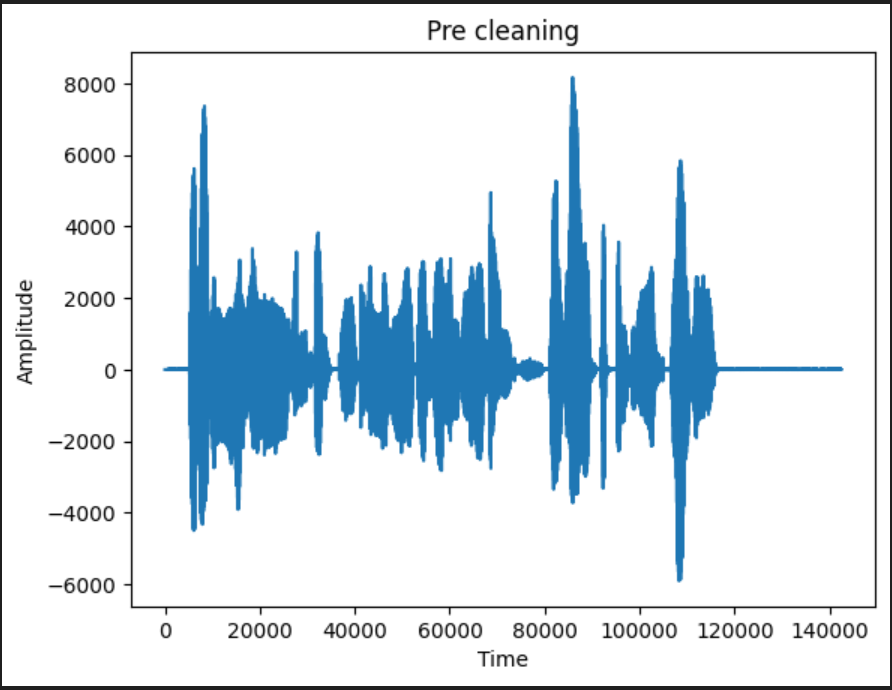
\includegraphics[width=\textwidth]{images/pre_cleaning.png}}
    \caption{Pre cleaning shape}
  \end{minipage}
  \hfill
  \begin{minipage}[b]{0.4\textwidth}
    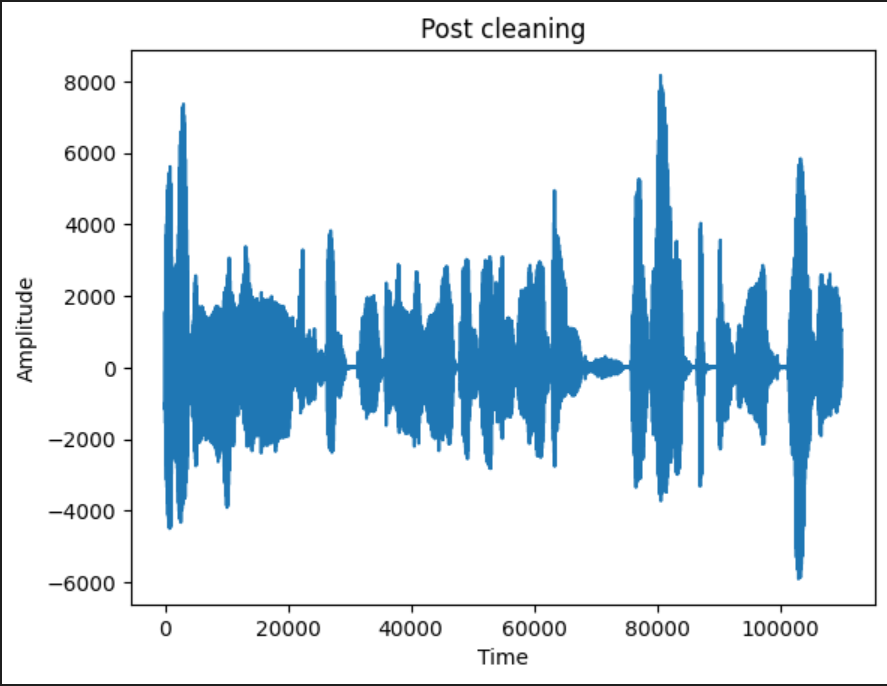
\includegraphics[width=\textwidth]{images/post_cleaning.png}
    \caption{Post cleaning shape}
  \end{minipage}
\end{figure}

\subsection{Statistics}
Before preprocessing our audio data into features for model training, we need to verify that the data is well-balanced across various attributes, such as label distribution, category balance, and uniformity in audio lengths. We looked at three statistics on the data: the total length of audios by language, the average length of audios by language, and the number of audio files by language.\\

\textbf{1.} The graphs below present the total length of audios by language.\\

\begin{figure}[!tbp]
  \centering
  \begin{minipage}[b]{0.4\textwidth}
    \includegraphics[width=\textwidth]{images/.png}}
    \caption{Pre cleaning shape}
  \end{minipage}
  \hfill
  \begin{minipage}[b]{0.4\textwidth}
    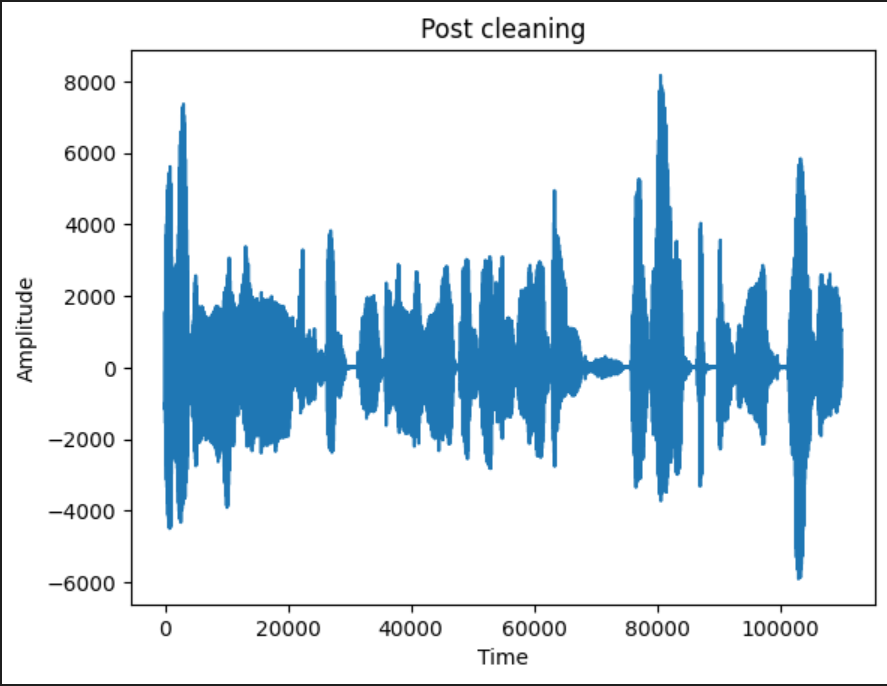
\includegraphics[width=\textwidth]{images/post_cleaning.png}
    \caption{Post cleaning shape}
  \end{minipage}
  \hfill
  \begin{minipage}[b]{0.4\textwidth}
    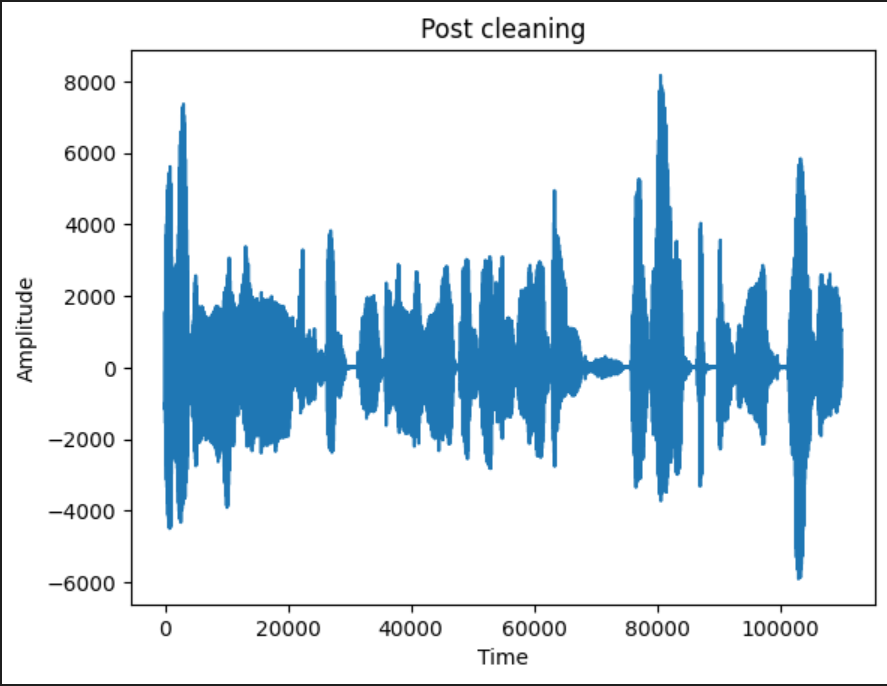
\includegraphics[width=\textwidth]{images/post_cleaning.png}
    \caption{Post cleaning shape}
  \end{minipage}
\end{figure}

We can notice that the training data as well as the test data are uniform. However, the validation data are not. To remedy this problem, it was necessary to merge the test and validation data. Here is the new graph obtained following the merger of these two data:\\

GRAPH\\

This merger (which we will consider as new test data) is much more significant than the validation data alone.\\
Therefore, the data are quite uniform in terms of the total length of audios by language.\\

\textbf{2.} The graphs below present the average length of audios by language for the two datasets.\\

FIGURES\\

It is possible to notice through the above graphs that the data are quite uniform among themselves.

\textbf{3.} The graphs below present the number of audio files by language for the two datasets.\\

FIGURES\\

It is possible to notice through the above graphs that the data are quite uniform among themselves.


\subsection{Data Preprocessing}
For the preprocessing of audio data, we use different attributes which are presented below.

\subsubsection{MFCCs}
The Mel Frequency Cepstral Coefficients are criticals in the sense that it allows capturing the different aspects that are unique to each spoken language. This makes it much easier to differentiate languages. To obtain the MFCCs, we first found the spectrum of power as a function of our audio file's frequencies from a Fast Fourier Transformation (FFT). Then, it was necessary to find the Mel Filter Banks (MFB) of the spectrum from which we obtain the frequency energies (weighted energy) passing through each filter of the bank. A logarithmic function will be applied to these energies. Finally, by applying a Discrete Cosine Transformation on the log-transformed energies, we obtain the MFCCs.\\

\subsubsection{Spectral Centroid}
This attribute is related to the clarity of the sound.

\subsubsection{Attribute Matrix}
After extracting raw features from the 
\section{Methodology}
\subsection{Why supervised Learning ?}

\subsection{Dimensionality reduction}
Before applying PCA or MDS, we wanted to see the relationship between features i.e. how strongly they are correlated. This correlation study would guide us in the dimensionality reduction algorithm we choose to apply to our. If some features are strongly correlated, PCA would be pertinent to be applied, as some features are linearly related. Even though our correlation study gave us pretty strong evidence of non-linear relationship between our features (meaning that MDS might be a better suit for our dataset), we opted to reduce dimensionality using PCA due to insufficient computing and memory. After applying PCA, with a maintained variance of $99\%$, we have $112$ features from the $151$ intial features. This means that the first $112$ principal components of the covariance matrix $\Sigma \in \mathbb{R}^{151 \times 151}$ , where $\forall i \in 1, \ldots, 151 \quad \forall j \in 1, \ldots, 151 \quad \sigma_{ij} \in \Sigma, \sigma_{ij} = COV(x_i, x_j)$, $99\%$ of the original dataset.

\subsection{SVM}
For this project, we use the library \textit{SVC} from \textit{sklearn}. This library use a non-linear SVM with a soft margin. Non-linear SVM with a soft margin is particularly useful when dealing with data that cannot be linearly separated in the original feature space. The inclusion of slack variables, \(\xi_i\), allows some data points to be on the incorrect side of the margin, providing a balance between the complexity of the model and its error minimization.\\

\noindent
\textbf{Formulation:}

For a dataset \(X \in \R^{n \times p} \) and a vector $y \in \{-1, 1\}^n$, the objective is to find $w$ such that the values returned by the functions $f(X) = sign(w^T\phi(x) + b)$ are correct for most samples.\\
SVC resolve the following problem :

\begin{equation}
\min_{w, b, \boldsymbol{\xi}} \left( \frac{1}{2} w^T w + \beta \sum_{i=1}^{n} \xi_i \right)
\end{equation}

subject to:
\[
y_i (w^T \phi(x_i) + b) \geq 1 - \xi_i
\]
\[
\xi_i \geq 0, \quad \forall i,
\]


\noindent
\textbf{Kernel Function}\\
Common choices for the kernel function \(K\) include:
- Polynomial: \(K(\mathbf{x}_i, \mathbf{x}_j) = (\gamma \mathbf{x}_i^T \mathbf{x}_j + r)^d\),
- Radial Basis Function (RBF): \(K(\mathbf{x}_i, \mathbf{x}_j) = \exp(-\gamma \|\mathbf{x}_i - \mathbf{x}_j\|^2)\),
- Sigmoid: \(K(\mathbf{x}_i, \mathbf{x}_j) = \tanh(\gamma \mathbf{x}_i^T \mathbf{x}_j + r)\).

\(\gamma\), \(r\), and \(d\) are parameters that can be tuned according to the specific data and problem requirements.


\subsection{Random Forest Classifier}

\section{Results}
\subsection{PCA}
 
\subsection{SVM vs Random Forest Classifier}

\section{Conclusion}

\newpage
\section{References}
\begin{itemize}
    \item \href{https://huggingface.co/datasets/common_language}{Data Source}
    \item \href{https://ietresearch.onlinelibrary.wiley.com/doi/full/10.1049/tje2.12082#:~:text=All\%20performance\%20metrics\%20gave\%20the,studies\%20use\%20only\%2013\%20MFCCs}{Number of MFCCs used in the code}
\end{itemize}


\section{Appendix}
\subsection{Definitions}
\textbf{Fast Fourier Transformation:}\label{fft}\\

\textbf{Filter:}\label{filter}\\

\textbf{Mel Filter Banks:}\label{mfb}\\

\textbf{Frequency Energy:}\label{freq-energy}\\

\textbf{Discrete Cosine Transformation:}\label{dct}

\end{document}
